\documentclass[11pt,letterpaper]{article}
\usepackage[latin1]{inputenc}
\usepackage[left=.5in,right=.5in,top=.5in,bottom=.5in]{geometry} 

%\usepackage[margin=.5in]{geometry} % see geometry.pdf on how to lay out the page. There's lots.
%\geometry{a4paper} % or letter or a5paper or ... etc
%\usepackage{fullpage}
\usepackage{amsfonts}
%\usepackage[margin=0.5in]{geometry}
% \geometry{landscape} % rotated page geometry
%\addtolength{\oddsidemargin}{-.875in}
%\addtolength{\evensidemargin}{-.875in}
%\addtolength{\textwidth}{1.75in}
%
%\addtolength{\topmargin}{-1.375in}
%\addtolength{\textheight}{1.875in}
\usepackage{framed}
\usepackage{makebox}
\usepackage{minibox}
\usepackage{graphicx}
\usepackage{caption}
%\usepackage{fullpage}
\usepackage{graphicx}
\usepackage{caption}
\usepackage{subcaption}
\usepackage{xcolor}
\usepackage{mdframed}
\usepackage{lipsum}
\usepackage{textcomp}
\usepackage{wrapfig}
\usepackage{setspace}
\usepackage{amsmath}
\usepackage{breqn}
\usepackage{amsmath}
\usepackage{amsfonts}
\usepackage{amssymb}
\usepackage{setspace}
\usepackage[colorlinks=true]{hyperref}
\usepackage{textcomp} 
\usepackage{multicol} 
 
\newcounter{NumberInTable}
\newcommand{\LTNUM}{\stepcounter{NumberInTable}{(\theNumberInTable)}}

\newcommand{\Laplace}[1]{\ensuremath{\mathcal{L}{\left[#1\right]}}}
\newcommand{\InvLap}[1]{\ensuremath{\mathcal{L}^{-1}{\left[#1\right]}}}
\DeclareMathOperator{\arcsec}{arcsec}
\DeclareMathOperator{\arccot}{arccot}
\DeclareMathOperator{\arccsc}{arccsc}

\colorlet{shadecolor}{blue!15}

\newtheorem{theorem}{Theorem}

\newenvironment{theo}
  {\begin{shaded}\begin{theorem}}
  {\end{theorem}\end{shaded}}

\usepackage{numprint}

%%% BEGIN DOCUMENT
\begin{document}
\begin{center}
\Large Math 252, 10.5, Area Polar Regions\normalsize\vspace{.1in}\\
\end{center}
\begin{enumerate}
\item \textbf{Area of a Sector} A sector of a circle is a region of the circle subtended by an angle $\theta$ \vspace{.1in}\\
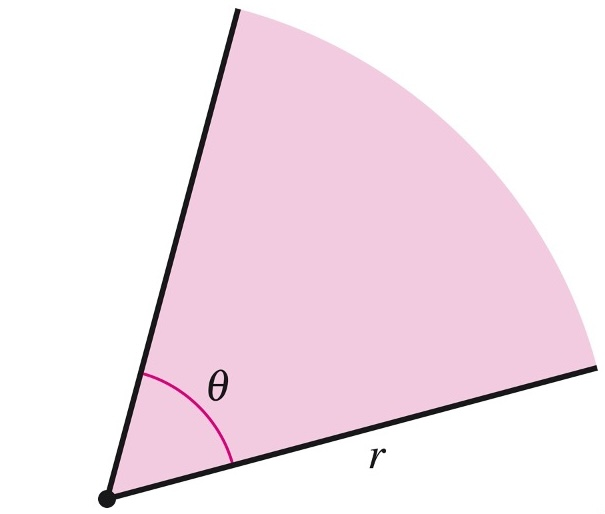
\includegraphics[scale=.3]{areapic1.jpg}

Since the sector represents the fraction $\dfrac{\theta}{2\pi}$ of the entire circle,
\begin{align*}
A_{\text{sector}}
&=\frac{\theta}{2\pi}\left(\pi r^{2}\right)\\
&=\frac{1}{2}r^{2}\theta.
\end{align*}
\item \textbf{Polar Regions}. Consider the function $r=f(\theta)$, for $\alpha <\theta<\beta$. \vspace{.05in}\\
\begin{figure}[h]
\begin{tabular}{ll}
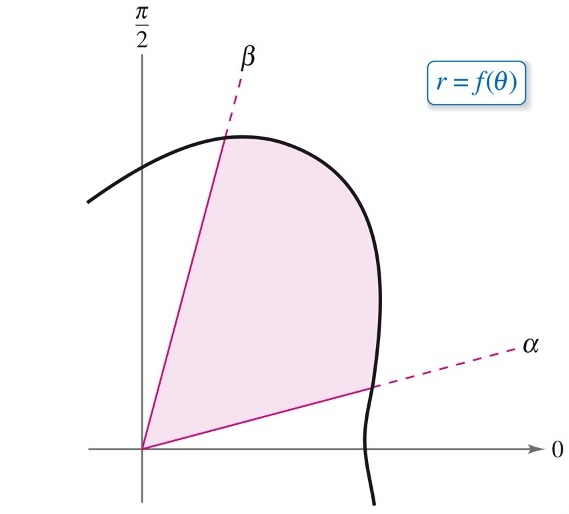
\includegraphics[scale=.3]{areapic2.jpg}
&
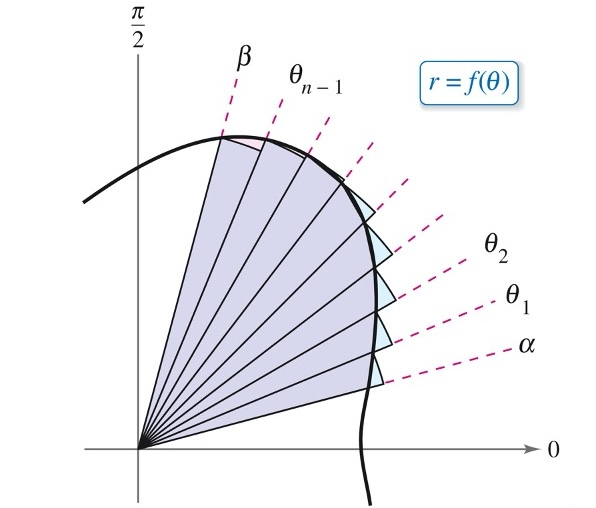
\includegraphics[scale=0.3]{areapic3.jpg}
\end{tabular}


\end{figure}

Partition the interval $[\alpha,\beta]$ into $n$ subintervals of width
$$\Delta\theta=\frac{\beta-\alpha}{n}.$$
On the $i$th subinterval, choose a sample angle $\theta_i^{*}$.  The corresponding thin polar region is approximately a sector with radius $f(\theta_i^{*})$ and central angle $\Delta\theta$, so
$$\Delta A_i\approx\frac{1}{2}\left[f(\theta_i^{*})\right]^2\Delta\theta.$$
Adding the areas of the sectors gives
$$A\approx\sum_{i=1}^{n}\frac{1}{2}\left[f(\theta_i^{*})\right]^2\Delta\theta.$$
Taking the limit as $n\to\infty$ gives the Riemann sum
\begin{align*}
A
&=\lim_{n\to\infty}\sum_{i=1}^{n}\frac{1}{2}\left[f(\theta_i^{*})\right]^2\Delta\theta\\
&=\int_{\alpha}^{\beta}\frac{1}{2}[f(\theta)]^{2}\,d\theta.
\end{align*}
%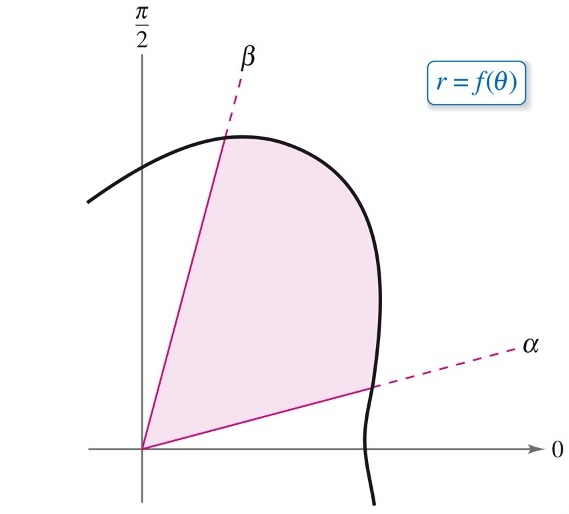
\includegraphics[scale=.3]{areapic2.jpg}\vspace{.1in}\\
%
%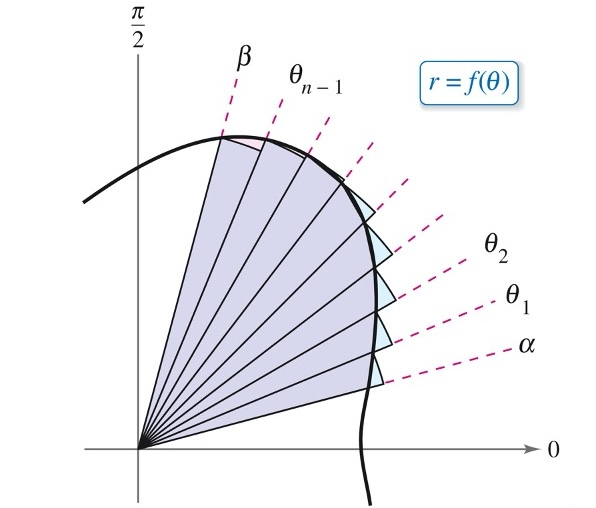
\includegraphics[scale=.3]{areapic3.jpg}\vspace{1in}
\item \textbf{Area of a Polar Region.}. If $f$ is continuous and nonnegative on the interval $[\alpha,\beta]$, $0<\beta-\alpha<2\pi$, then the area of the region of the area bounded between $\alpha$ and $\beta$ is given by,
$$\int_{\alpha}^{\beta}\frac{1}{2}[f(\theta)]^{2}\, d\theta$$
\newpage
\item \textbf{Main Tool for Integration.}. We use the half-angle formulas from trigonometry
$$\cos^{2}\theta=\frac{\cos 2\theta+1}{2}\,\,\,\,\,\sin^{2}\theta=\frac{1-\cos 2\theta}{2}$$
\item \textbf{Example 1:} Determine the area one petal of the graph of $r=3\cos 3\theta$.\\
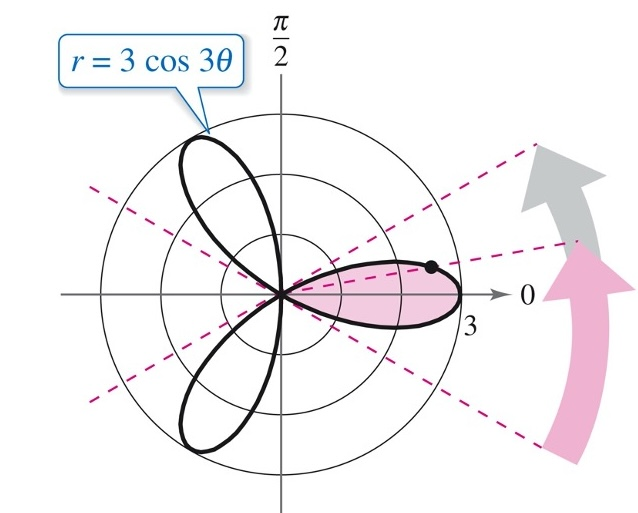
\includegraphics[scale=.25]{areapic4.jpg}

The petal centered on the polar axis begins and ends where $r=0$:
$$3\cos 3\theta=0\quad\Longrightarrow\quad \theta=-\frac{\pi}{6},\frac{\pi}{6}.$$
Therefore,
\begin{align*}
A
&=\frac{1}{2}\int_{-\pi/6}^{\pi/6}(3\cos 3\theta)^2\,d\theta\\
&=\frac{9}{2}\int_{-\pi/6}^{\pi/6}\cos^2 3\theta\,d\theta\\
&=\frac{9}{2}\int_{-\pi/6}^{\pi/6}\frac{1+\cos 6\theta}{2}\,d\theta\\
&=\frac{9}{4}\left[\theta+\frac{1}{6}\sin 6\theta\right]_{-\pi/6}^{\pi/6}\\
&=\boxed{\frac{3\pi}{4}}.
\end{align*}
\newpage
\item \textbf{Example 2:} Determine the area of the outter loop of the lima\c{c}on with inner loop given by $r=1-2\sin \theta$.\\
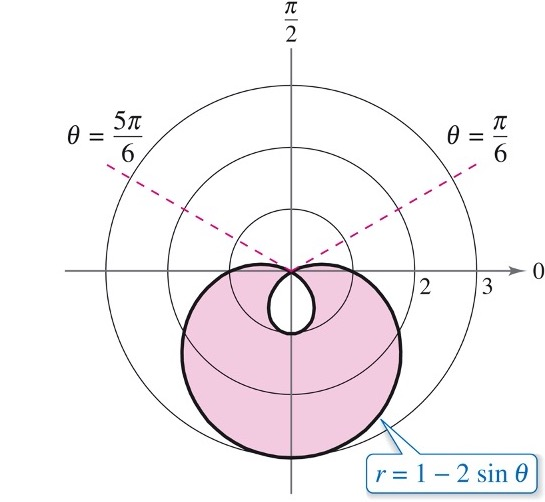
\includegraphics[scale=.35]{areapic5.jpg}

First determine where the curve passes through the pole:
\begin{align*}
1-2\sin\theta&=0\\
\sin\theta&=\frac{1}{2},
\end{align*}
so $\theta=\dfrac{\pi}{6}$ and $\theta=\dfrac{5\pi}{6}$.  The outer loop is traced from $\theta=\dfrac{5\pi}{6}$ to $\theta=\dfrac{13\pi}{6}$.  Thus,
\begin{align*}
A
&=\frac{1}{2}\int_{5\pi/6}^{13\pi/6}(1-2\sin\theta)^2\,d\theta\\
&=\frac{1}{2}\int_{5\pi/6}^{13\pi/6}\left(1-4\sin\theta+4\sin^2\theta\right)\,d\theta\\
&=\frac{1}{2}\int_{5\pi/6}^{13\pi/6}\left(3-4\sin\theta-2\cos 2\theta\right)\,d\theta\\
&=\frac{1}{2}\left[3\theta+4\cos\theta-\sin 2\theta\right]_{5\pi/6}^{13\pi/6}\\
&=\boxed{2\pi+\frac{3\sqrt{3}}{2}}.
\end{align*}
\newpage
\item \textbf{Example 3:} Determine the area of the region bounded between the cardioid $r=2-2\cos\theta$ and the circle $r=-6\cos \theta$.\\
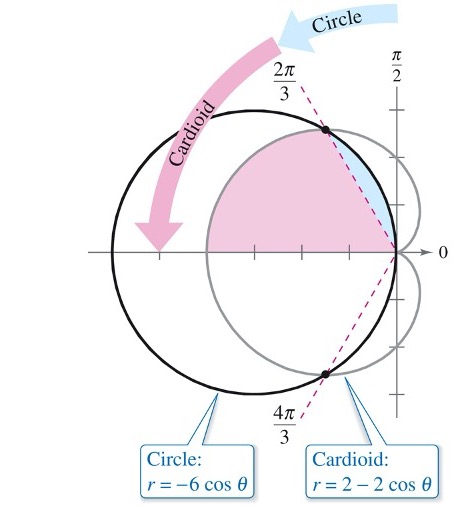
\includegraphics[scale=.35]{areapic7.jpg}

Find the angles at which the curves intersect:
\begin{align*}
2-2\cos\theta&=-6\cos\theta\\
2&=-4\cos\theta\\
\cos\theta&=-\frac{1}{2}.
\end{align*}
Thus, the curves intersect at $\theta=\dfrac{2\pi}{3}$ and $\theta=\dfrac{4\pi}{3}$.  By symmetry about the polar axis, we may find the area above the axis and double it.  On $\left[\dfrac{\pi}{2},\dfrac{2\pi}{3}\right]$, the circle is the inner curve, and on $\left[\dfrac{2\pi}{3},\pi\right]$, the cardioid is the inner curve.  Therefore,
\begin{align*}
A
&=2\left[\frac{1}{2}\int_{\pi/2}^{2\pi/3}(-6\cos\theta)^2\,d\theta
+\frac{1}{2}\int_{2\pi/3}^{\pi}(2-2\cos\theta)^2\,d\theta\right]\\
&=\int_{\pi/2}^{2\pi/3}36\cos^2\theta\,d\theta
+\int_{2\pi/3}^{\pi}(2-2\cos\theta)^2\,d\theta\\
&=2\left[\left(\frac{3\pi}{2}-\frac{9\sqrt{3}}{4}\right)
+\left(\pi+\frac{9\sqrt{3}}{4}\right)\right]\\
&=\boxed{5\pi}.
\end{align*}
\end{enumerate}
\end{document}




















